\section{拓扑学 \\Topology}

为了简洁性, 此处一些概念名词指代的是单个元素, 而定义和示意图表示的是所有元素组成的集合.

\mydefboxillus{$E$ (a sample set)}{$E$ (示例集合)}{
	$\begin{aligned}
		\mathbb{R}^2\supset E={}&\hphantom{{}\cup{}}\left\lbrace(x,y)\in\mathbb{R}^2\relmiddle|x^2+y^2\leqslant 1,\, y\geqslant 0\right\rbrace\\
		&\cup{}\left\lbrace(x,y)\in\mathbb{R}^2\relmiddle|x^2+y^2<1,\, y<0\right\rbrace\\
		&\cup{}\left\lbrace(x,y)\in\mathbb{R}^2\relmiddle|x=1.5,\, 0<y<0.5\right\rbrace\\
		&\cup{}\left\lbrace(1.5,-0.5)\in\mathbb{R}^2\right\rbrace.
	\end{aligned}$
}{
	
\begin{tikzpicture}[very thick]
		\fill[color=white] (-1.2,-1.2) rectangle (1.8,1.2);
		\fill[color=teal,opacity=0.4] (0,0) circle[radius=1];
		\draw[color=teal,opacity=0.8] (1,0) arc[radius=1,start angle=0,end angle=180];
		\draw[color=black,opacity=0.8,dashed,thin] (-1,0) arc[radius=1,start angle=180,end angle=360];
		\draw[color=teal,opacity=0.8] (1.5,0.5) -- (1.5,0);
		\fill[color=teal,opacity=0.8] (1.5,-0.5) circle[radius=1pt];
	\end{tikzpicture}
}

\mydefboxillus{accumulation point | limit point}{聚点 | 极限点}{
	$E'=\left\lbrace\boldsymbol{x}\relmiddle|\forall\delta>0,\ U_0(\boldsymbol{x},\,\delta)\cap E\neq\varnothing\right\rbrace$.
}{
	
\begin{tikzpicture}[very thick]
		\fill[color=white] (-1.2,-1.2) rectangle (1.8,1.2);
		\fill[color=teal,opacity=0.4] (0,0) circle[radius=1];
		\draw[color=teal,opacity=0.8] (1,0) arc[radius=1,start angle=0,end angle=180];
		\draw[color=teal,opacity=0.8,dashed] (-1,0) arc[radius=1,start angle=180,end angle=360];
		\draw[color=teal,opacity=0.8] (1.5,0.5) -- (1.5,0);
		\fill[color=black,opacity=0.8] (1.5,-0.5) circle[radius=0.5pt];
	\end{tikzpicture}
}

\mydefboxillus{closure}{闭包}{
	$\overline{E}=E\cup E'$.
}{
	
\begin{tikzpicture}[very thick]
		\fill[color=white] (-1.2,-1.2) rectangle (1.8,1.2);
		\fill[color=teal,opacity=0.4] (0,0) circle[radius=1];
		\draw[color=teal,opacity=0.8] (1,0) arc[radius=1,start angle=0,end angle=180];
		\draw[color=teal,opacity=0.8,dashed] (-1,0) arc[radius=1,start angle=180,end angle=360];
		\draw[color=teal,opacity=0.8] (1.5,0.5) -- (1.5,0);
		\fill[color=teal,opacity=0.8] (1.5,-0.5) circle[radius=1pt];
	\end{tikzpicture}
}

\mydefboxillus{interior}{内部}{
	$E^\circ=\left\lbrace\boldsymbol{x}\relmiddle|\exists\delta>0,\ U(\boldsymbol{x},\,\delta)\subset E\right\rbrace$.

	$E^\circ=\left\lbrace\boldsymbol{x}\relmiddle|\exists\delta>0,\ U(\boldsymbol{x},\,\delta)\cap E^c=\varnothing\right\rbrace$.
}{
	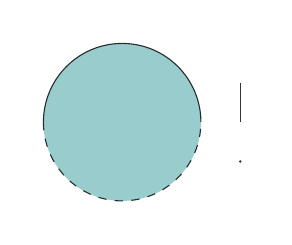
\begin{tikzpicture}[very thick]
		\fill[color=white] (-1.2,-1.2) rectangle (1.8,1.2);
		\fill[color=teal,opacity=0.4] (0,0) circle[radius=1];
		\draw[color=black,opacity=0.8,thin] (1,0) arc[radius=1,start angle=0,end angle=180];
		\draw[color=black,opacity=0.8,dashed,thin] (-1,0) arc[radius=1,start angle=180,end angle=360];
		\draw[color=black,opacity=0.8,thin] (1.5,0.5) -- (1.5,0);
		\fill[color=black,opacity=0.8] (1.5,-0.5) circle[radius=0.5pt];
	\end{tikzpicture}
}

\mydefboxillus{exterior}{外部}{
	$(E^c)^\circ=\left\lbrace\boldsymbol{x}\relmiddle|\exists\delta>0,\ U(\boldsymbol{x},\,\delta)\cap E=\varnothing\right\rbrace$.

	$(E^c)^\circ=\left\lbrace\boldsymbol{x}\relmiddle|\exists\delta>0,\ U(\boldsymbol{x},\,\delta)\subset E^c\right\rbrace$.
}{
	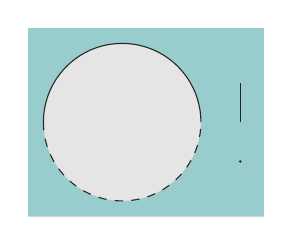
\begin{tikzpicture}[very thick]
		\fill[color=white] (-1.2,-1.2) rectangle (1.8,1.2);
		\begin{scope}
			\clip
				(-1.2,-1.2) rectangle (1.8,1.2)
				(0,0) circle[radius=1]
			;
			\fill[color=teal,opacity=0.4] (-1.2,-1.2) rectangle (1.8,1.2);
		\end{scope}
		\fill[color=black,opacity=0.1] (0,0) circle[radius=1];
		\draw[color=black,opacity=0.8,thin] (1,0) arc[radius=1,start angle=0,end angle=180];
		\draw[color=black,opacity=0.8,dashed,thin] (-1,0) arc[radius=1,start angle=180,end angle=360];
		\draw[color=black,opacity=0.8,thin] (1.5,0.5) -- (1.5,0);
		\fill[color=black,opacity=0.8] (1.5,-0.5) circle[radius=0.5pt];
	\end{tikzpicture}
}

\mydefboxillus{boundary}{边界}{
	$\partial E=\left\lbrace\boldsymbol{x}\relmiddle|\forall\delta>0,\ (U(\boldsymbol{x},\,\delta)\cap E\neq\varnothing)\wedge(U(\boldsymbol{x},\,\delta)\cap E^c\neq\varnothing)\right\rbrace$.

	$\partial E=\mathbb{R}^n\setminus(E^\circ\cup(E^c)^\circ)$.
}{
	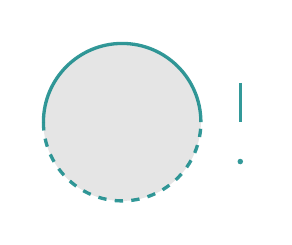
\begin{tikzpicture}[very thick]
		\fill[color=white] (-1.2,-1.2) rectangle (1.8,1.2);
		\fill[color=black,opacity=0.1] (0,0) circle[radius=1];
		\draw[color=teal,opacity=0.8] (1,0) arc[radius=1,start angle=0,end angle=180];
		\draw[color=teal,opacity=0.8,dashed] (-1,0) arc[radius=1,start angle=180,end angle=360];
		\draw[color=teal,opacity=0.8] (1.5,0.5) -- (1.5,0);
		\fill[color=teal,opacity=0.8] (1.5,-0.5) circle[radius=1pt];
	\end{tikzpicture}
}
